\documentclass[numbers=noenddot,10pt,a4paper]{scrartcl}
\usepackage[greek,ngerman]{babel}
\usepackage[T1]{fontenc}
\usepackage[utf8]{inputenc}
\usepackage{fullpage}
\usepackage{libertine}
\usepackage{ziffer}
\usepackage{graphicx}
\usepackage{units}
%\usepackage{wasysym}
\usepackage{amsmath}
\usepackage{amssymb}
\usepackage{wrapfig}
\usepackage{esint}
\usepackage{float}
\usepackage{wrapfig}
\usepackage[font=small]{caption}
\usepackage{subcaption}

\renewcommand{\thefigure}{Abb. \arabic{figure}}

\captionsetup[wrapfigure]{name=}
\captionsetup[figure]{name=}
\newcommand{\degree}{^\circ}
\newcommand{\diff}{\textnormal{d}}
\newcommand{\tenpo}[1]{\cdot 10^{#1}}
\newcommand{\greek}[1]{\greektext#1\latintext}
\newcommand{\indx}[1]{_\text{#1}}

\title{Protokoll: Astabiler Multivibrator}
\author{Tom Kranz, Philipp Hacker}
\date{\today}

\begin{document}
%\setcounter{page}{2}
%\setcounter{section}{1}
\maketitle
\vspace*{\fill}
\tableofcontents
\vfill
\newpage
\section{Vorbereitung}
\subsection{Schaltskizzen}
\begin{figure}[H]
\centering
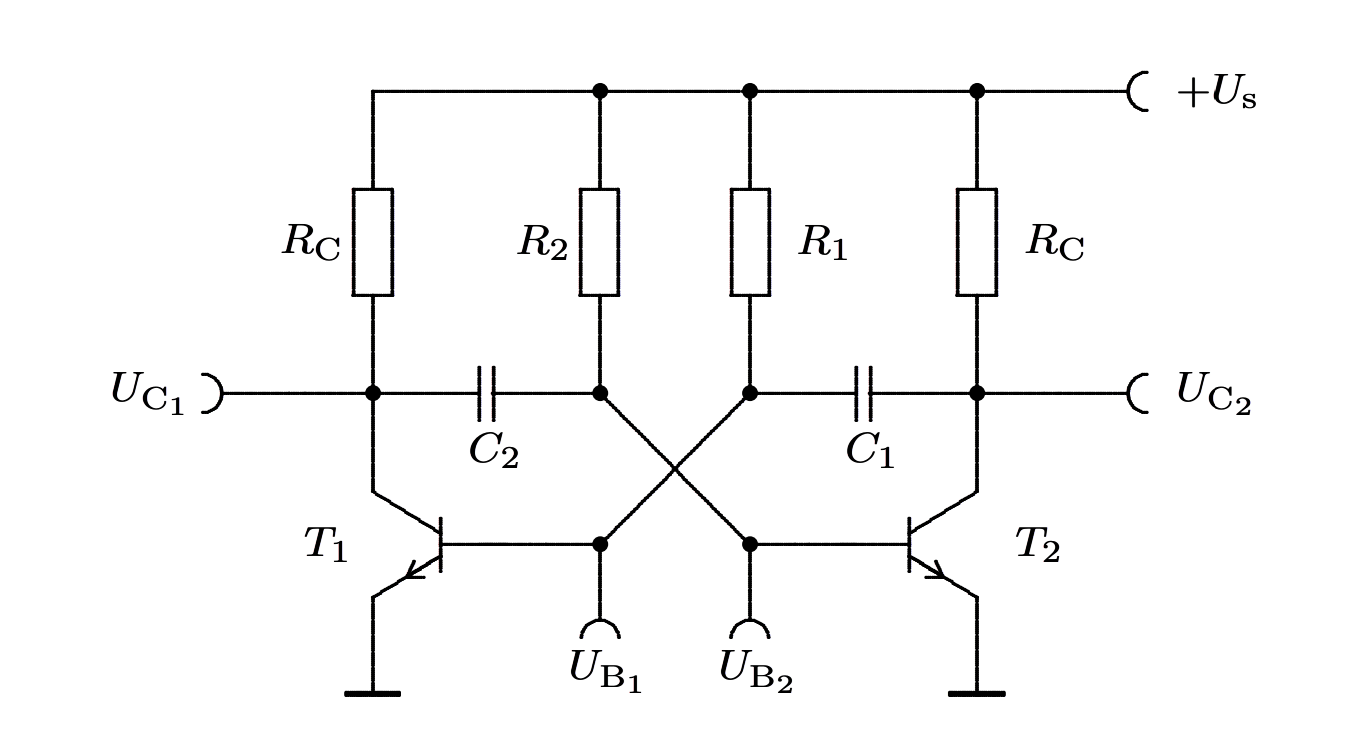
\includegraphics[width=0.75\textwidth]{schaltskizze1}
\caption{Astabiler Multivibrator}
\end{figure}
\begin{figure}[H]
\centering
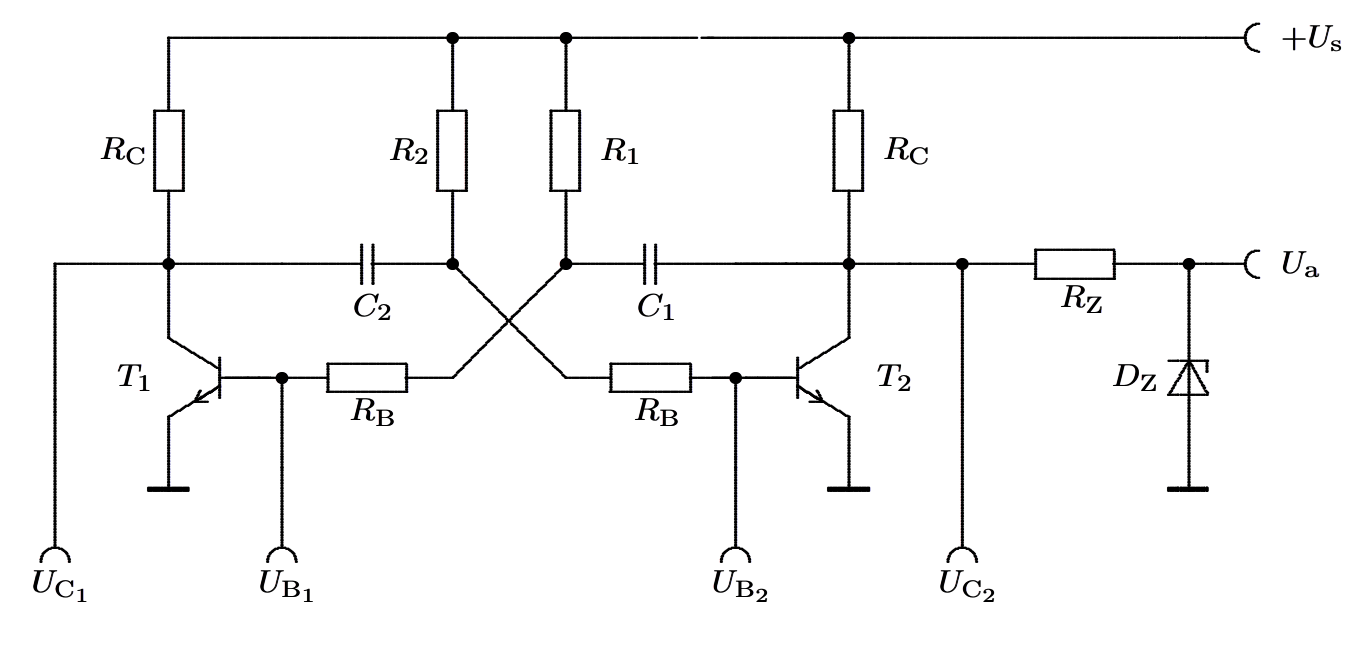
\includegraphics[width=0.75\textwidth]{schaltskizze2}
\caption{Astabiler Multivibrator mit Transistorvorwiderständen und Zener-Diode über dem Ausgang}
\end{figure}
\subsection{Berechnungsaufgabe 1 - korrigierte Frequenz}
Es gilt, dass
\begin{align}
U\indx{B}(t=0)=U\indx{BE;sat}-(U\indx{S}-U\indx{CE;sat}) \quad \text{und} \quad U\indx{B}(t\indx{2})=U\indx{BE;Schw} \, .
\end{align}
Somit folgt für die Funktion der Basisspannung $U\indx{B}(t)$, mit den Zeitkostanten $\tau_i=R_i\cdot C_i$:
\begin{align}
U\indx{B}(t)=U\indx{B}(t=0)+(U\indx{S}-U\indx{B}(t=0))\cdot\left(1-\exp\left(-\frac{t}{\tau\indx{2}}\right)\right) \, .
\end{align}
Zum Zeitpunkt $t\indx{2}$ ist also
\begin{align}
U\indx{BE;Schw}=U\indx{B}(t=0)+(U\indx{S}-U\indx{B}(t=0))\cdot\left(1-\exp\left(-\frac{t\indx{2}}{\tau\indx{2}}\right)\right) \, .
\end{align}
Nach Umformung analog zur Praktikumsanleitung, Gleichungen (1.3) und folgende, steht:
\begin{align}
t\indx{2}=-\tau\indx{2}\ln\left(\frac{2\cdot U\indx{S}-U\indx{BE;sat}-U\indx{CE;sat}}{U\indx{S}-U\indx{BE;Schw}}\right)
\end{align}
Für den Zeitpunkt $t'=t\indx{3}-t\indx{2}$ gilt ähnliches, wobei $t\indx{3}$ der Periodendauer $T$ entspricht. Somit folgt
\begin{align}
t_3-t_2=\tau_1 \ln\left(\frac{2\cdot U\indx{S}-U\indx{BE;sat}-U\indx{CE;sat}}{U\indx{S}-U\indx{BE;Schw}}\right) \, .
\end{align}
Schließlich steht
\begin{align}
t_3=\frac{1}{f}=(\tau_1+\tau_2)\ln\left(\frac{2\cdot U\indx{S}-U\indx{BE;sat}-U\indx{CE;sat}}{U\indx{S}-U\indx{BE;Schw}}\right) \, . \label{eq:freq}
\end{align}
\subsection{Berechnung 2 - Dimensionierung}
Aufgabe war es, den astabilen Multivibrator für eine Frequenz von ungefähr $\unit[5]{kHz}$ bei einer Speisespannung von $\unit[10]{V}$ zu dimensionieren. Dafür sollten $R_1=R_2$ und $C_1=C_2$ angepasst werden. Zu beachten war, dass die Transistoren voll durchgesteuert werden konnten, also ein Basisstrom von mindestens $\unit[0,1]{mA}$ erreicht würde. Deswegen durften $R_1$ und $R_2$ nicht beliebig groß gewählt werden. Wegen dem maximal zulässigen Kollektorstrom von $\unit[0,5]{A}$ mussten die Widerstände $R\indx{C}$ mindestens $\unit[20]{\Omega}$ betragen. Des Weiteren ist $R\indx{C}$ von oben durch die Anforderung beschränkt, dass im Messpunkt $U\indx{C2}$ die Spannung nicht zusammenbrechen sollte. Um die Bauteile nicht an ihre Grenzen zu bringen, wurden die Widerstände vorsichtig geplant: $R\indx{C}\approx\unit[500]{\Omega}$ und $R_1=R_2\approx\unit[10]{k\Omega}$, woraus sich dann auch die Kapazitäten zu etwa $C_1=C_2\approx\unit[20]{nF}$ ergaben. Für den Transistorvorwiderstand musste darauf geachtet werden, dass der Basisstrom weiterhin zum Durchsteuern ausreicht -- das wurde durch die Überlegung $R\indx{B}<\frac{U\indx{S}}{I\indx{B;min}}\approx\unit[100]{k\Omega}$ gelöst. Letztlich wurden aus dem vorhandenen Sortiment folgende Bauteile ausgewählt:
\begin{table}[H]
\caption{verwendete Bauelemente}
\vspace{-1em}
\begin{align*}
\begin{array}{c|c|c|c}
 R\indx{C} & R_1\approx R_2 & C_1\approx C_2 & R\indx{B} \\ 
\hline \unit[557]{\Omega} & \unit[9,92]{k\Omega} & \unit[22]{nF} & \unit[1]{k\Omega}
\end{array} 
\end{align*}
\end{table}
\section{Durchführung}
\subsection{Messgeräte}
Für die Messungen am astabilen Multivibrator und für die Aufnahme der Oszillogramme verwendeten wir das Oszilloskop HAMEG HM1508. Zur gesonderten Messung der Widerstände, Kapazitäten und Schwellspannungen wurde das Multimeter VOLTCRAFT VC920 benutzt. Die Stromversorgung erfolgte über eine Tektronix PS280. Weiterhin waren die Transistoren SF129 und die Zener-Diode SZX21/5,1 gegeben.
\subsection{Oszillogramme}
\begin{figure}[H]
\centering
\begin{subfigure}[b]{0.66\textwidth}
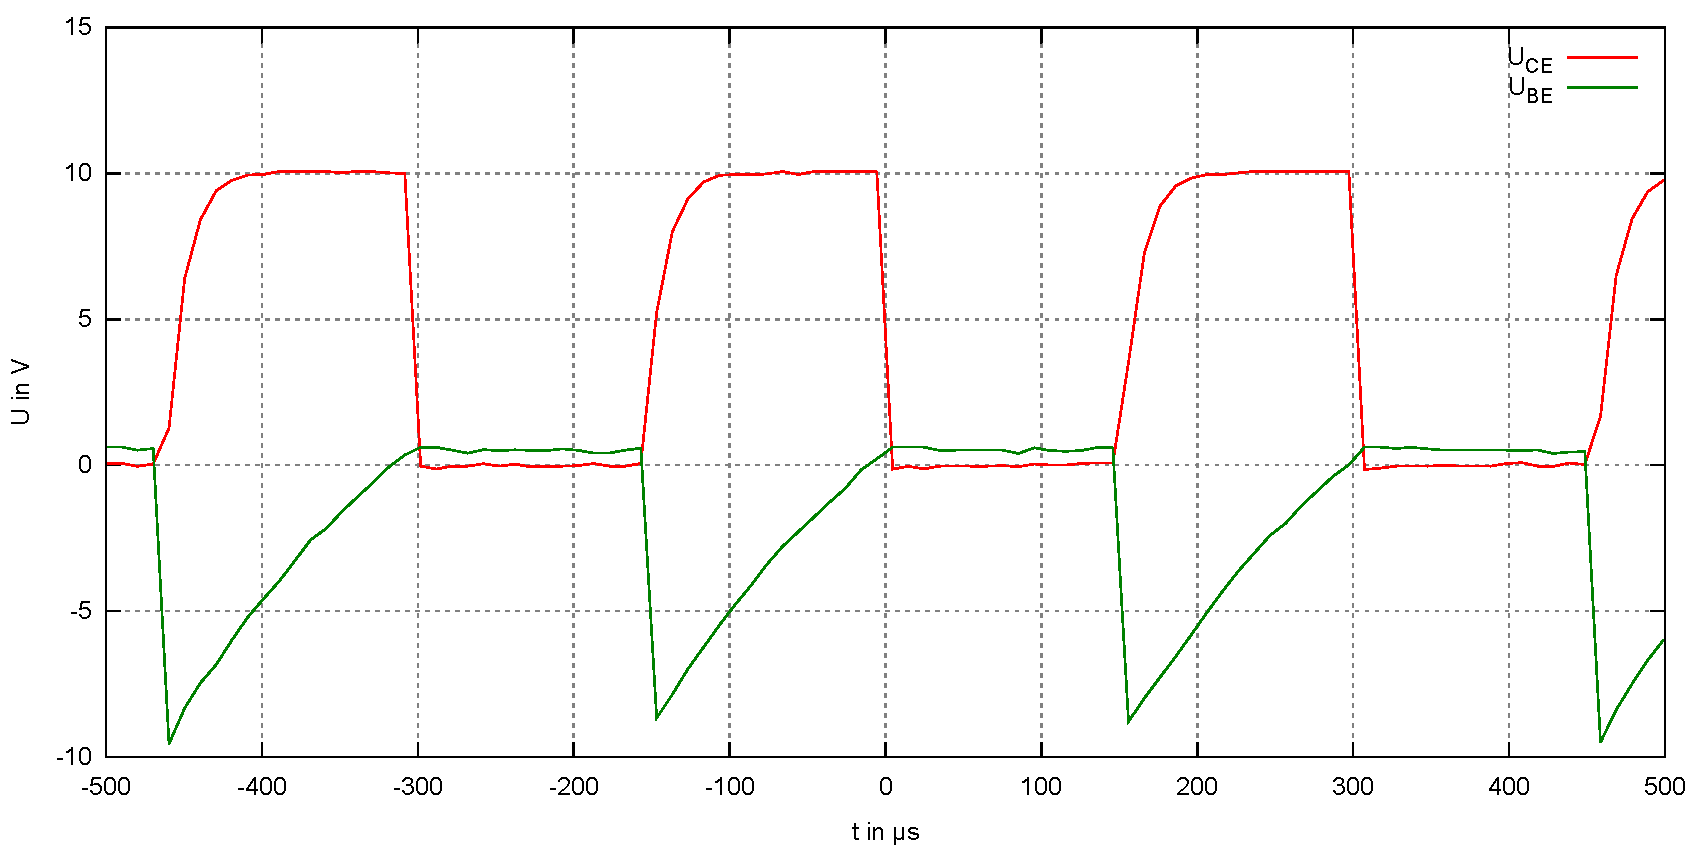
\includegraphics[width=\textwidth]{oszillo1.pdf}
\caption{aus Messwerten, geglättet}
\end{subfigure}
\begin{subfigure}[b]{0.33\textwidth}
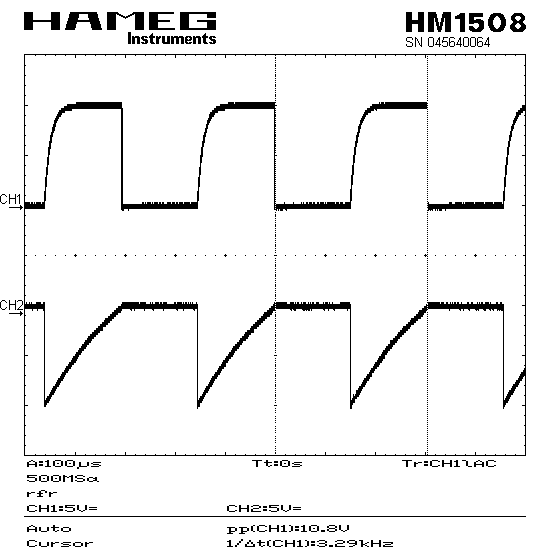
\includegraphics[width=\textwidth]{SCR00000.png}
\caption{unbearbeitet}
\end{subfigure}
\caption{Oszillogramme -- Messaufgabe 1}
\end{figure}

\begin{figure}[H]
\centering
\begin{subfigure}[b]{0.66\textwidth}
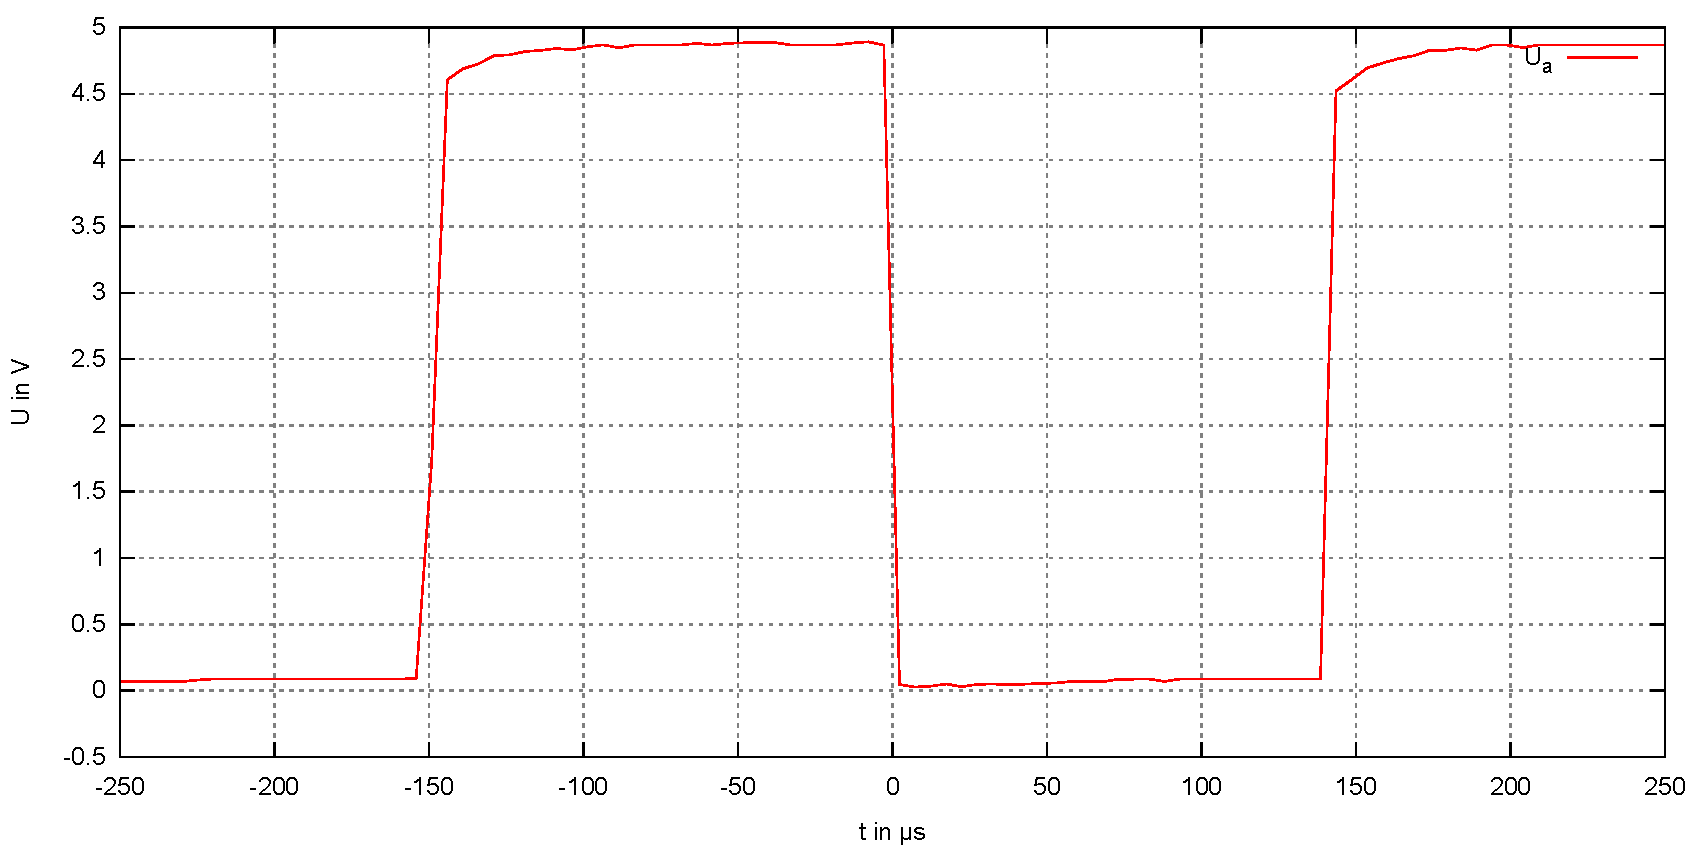
\includegraphics[width=\textwidth]{oszillo2.pdf}
\caption{aus Messwerten, geglättet}
\end{subfigure}
\begin{subfigure}[b]{0.33\textwidth}
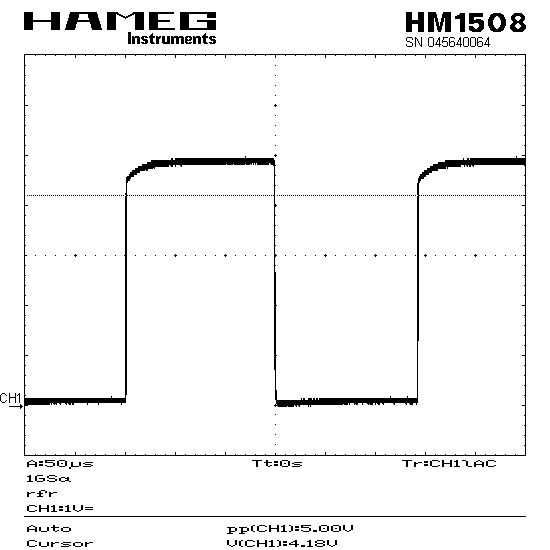
\includegraphics[width=\textwidth]{SCR00003.png}
\caption{unbearbeitet}
\end{subfigure}
\caption{Oszillogramme -- Messaufgabe 4}
\end{figure}
\subsection{Separate Messergebnisse}
Während der "`vollen Durchsteuerung"' der Transistoren (fehlender Widerstand $R_1$ bzw. $R_2$) wurde mit dem Multimeter die Basis-Emitter- und die Kollektor-Emitter-Spannung gemessen. Diese entsprechen dann gerade den jeweiligen Sättigungsspannungen $U\indx{CE;sat}=\unit[77]{mV}$ und $U\indx{BE;sat}=\unit[689]{mV}$. Für Gleichung (\ref{eq:freq}) benötigten wir zudem die Basis-Emitter-Schwellspannung, welche mit der Diodenprüffunktion des Multimeters zu $U\index{BE;Schw}=\unit[534]{mV}$ bestimmt wurde. \\
Außerdem war es auch oszillographisch möglich, die Sättigungsspannungen zumindest näherungsweise zu bestimmen. Hierfür ergaben sich die folgenden Oszillogramme, auf denen die Werte eingetragen wurden:
\begin{figure}[H]
\centering
\begin{subfigure}[b]{0.4\textwidth}
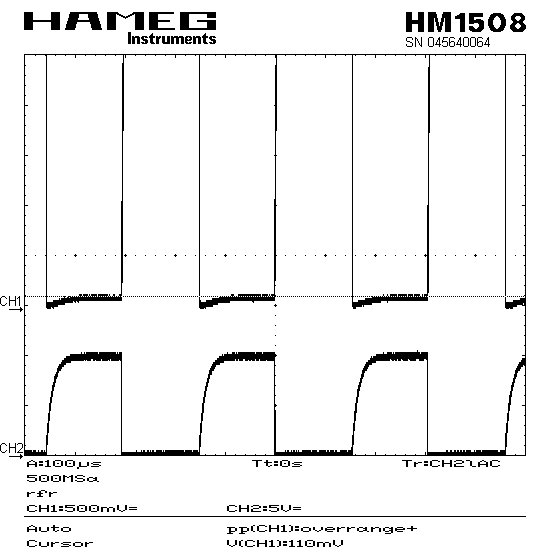
\includegraphics[width=\textwidth]{SCR00001.png}
\caption{$U\indx{CE;sat}$}
\end{subfigure}
\begin{subfigure}[b]{0.4\textwidth}
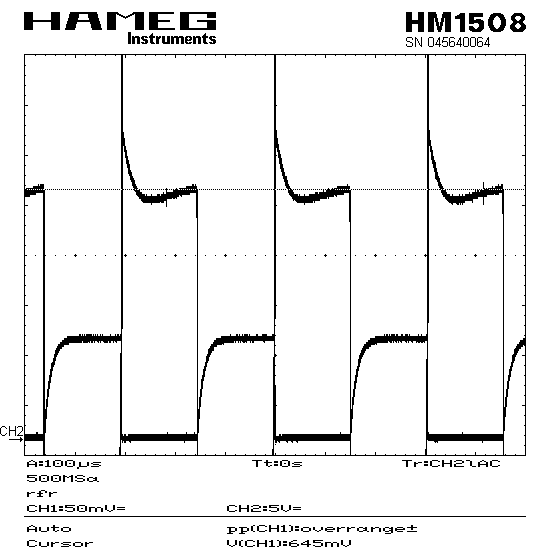
\includegraphics[width=\textwidth]{SCR00002.png}
\caption{$U\indx{BE;sat}$}
\end{subfigure}
\caption{Messaufgabe 2, oszillographisch}
\end{figure}
\begin{figure}[H]
\centering
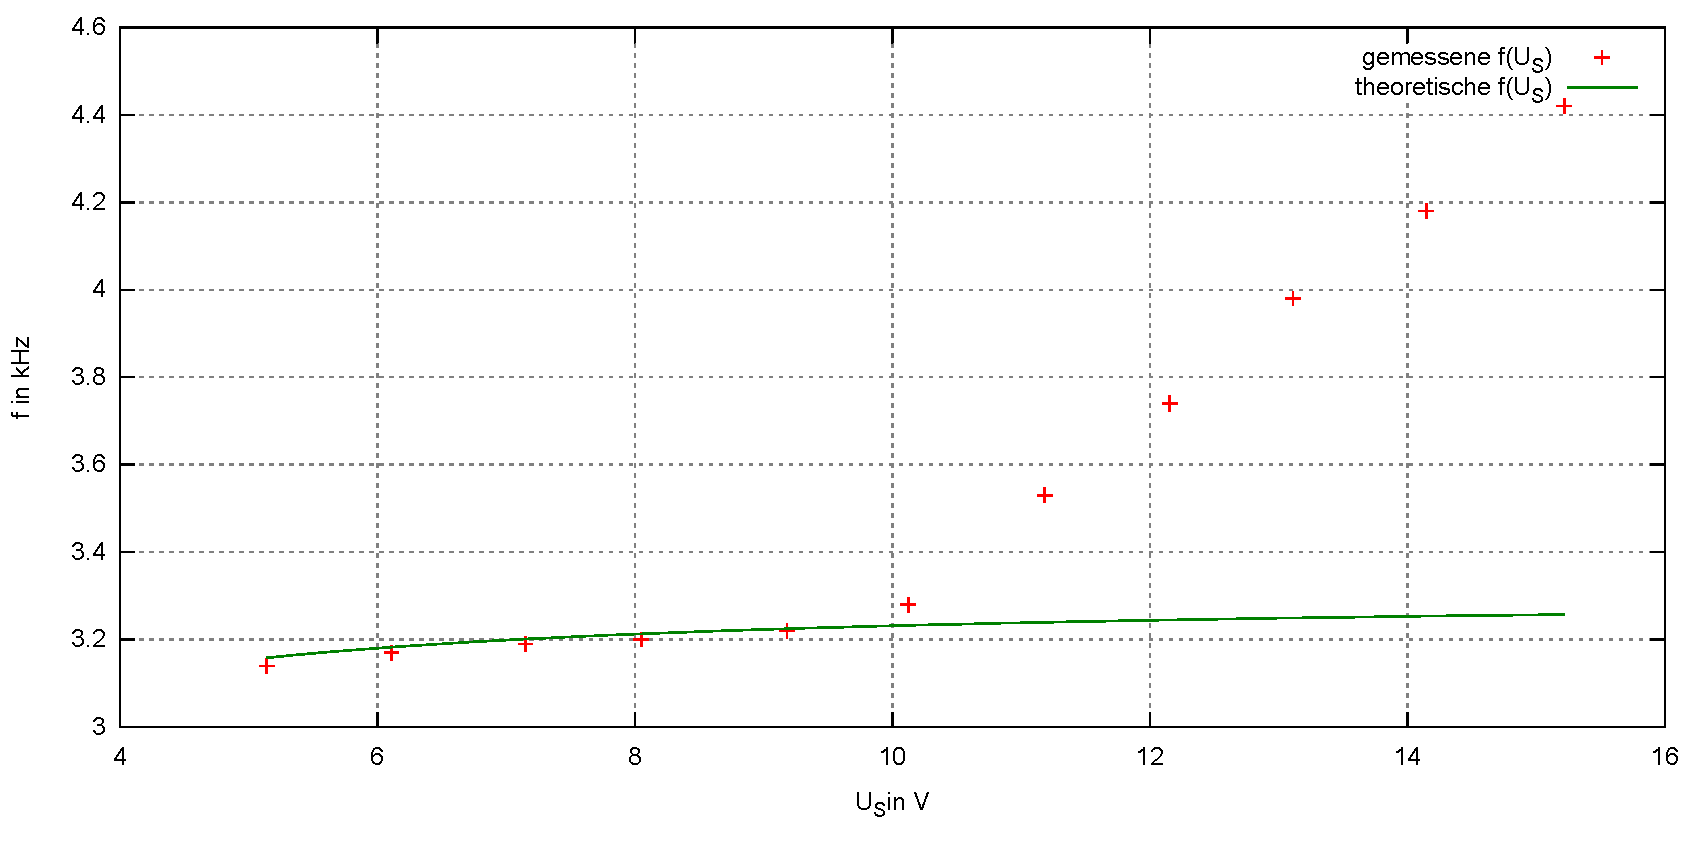
\includegraphics[width=0.8\textwidth]{messwerteUf.pdf}
\caption{$f(U\indx{S})$-Diagramm -- Messaufgabe 5}
\end{figure}
\section{Auswertung}
\subsection{Messaufgabe 1}
Das Oszillogramm zeigt den erwarteten zeitlichen Verlauf der Spannungen und gibt sogar Aufschluss über die Frequenz des symmetrischen Multivibrators. Die Schaltung erfüllt also ihren Zweck.
\subsection{Messaufgabe 4}
Wenn $C_2$ durch den Strom $I\indx{B2}$ entladen wird, fällt über $R\indx{B}$ eine Spannung $R\indx{B}\cdot I\indx{B2}$ ab. Dieser Spannungsabfall lässt die Basis-Emitter-Spannung schneller unter den Schwellwert fallen und den Transistor $T_2$ früher sperren. Gleiches gilt für $T_1$, da die Schaltung symmetrisch ist. Schließlich "`schneidet"' die Zener-Diode das Ausgangssignal am Messpunkt $U\indx{a}$ ab, was einen glattereren Rechteckimpuls zur Folge hat.
\subsection{Messaufgabe 5}
Die Messung stimmt nicht mit den theoretischen Überlegungen der Vorbereitung überein. Lediglich bei kleinen Spannungen kommen sich Experiment und Voraussage nahe.
\section{Anhang}
Die originalen Messwert-Aufzeichnungen liegen bei.
\end{document}